\documentclass[conference]{IEEEtran}
\usepackage{cite}
\usepackage{amsmath,amssymb,amsfonts}
\usepackage{graphicx}
\usepackage{textcomp}
\usepackage{xcolor}
\usepackage{booktabs}
\usepackage{multirow}
\usepackage{url}
\usepackage{hyperref}

\graphicspath{{../paper_figures/}}

\begin{document}

\title{TrustBench: Evaluating Large Language Models on Security Compliance Auditing}

\author{\IEEEauthorblockN{Varun Gurnaney}
\IEEEauthorblockA{\\varun@delve.co}}

\maketitle

\begin{abstract}
This paper presents TrustBench, a benchmark for evaluating large language models on security compliance auditing tasks. The benchmark comprises 20 tasks across 8 SOC~2 Trust Service Criteria controls at five difficulty levels, ranging from single-document gap detection to materiality judgment under ambiguity. Each task presents models with synthetic audit evidence---policies, configurations, access logs, and exception registers---containing planted compliance gaps. Scoring is deterministic: keyword-based detection for simple tasks, F1 for tasks involving red herrings and noise documents. We evaluate six models from Anthropic and OpenAI across all 20 tasks (120 runs). Claude Sonnet~4.6 achieves the highest average score at 82\%, followed by Opus~4.7 (72\%) and GPT-5.5 (71\%). Three judgment tasks average below 28\% across all models, suggesting that professional compliance judgment remains beyond current capabilities. We identify a systematic scoring limitation: F1 penalizes models that report legitimate findings beyond the planted ground truth, favoring concise models over thorough ones. The benchmark schema is framework-agnostic and extensible to ISO~27001, HIPAA, and PCI-DSS without changes to the evaluation harness. Code and data are available at \url{https://github.com/varungurnaney/trustbench}.
\end{abstract}

\begin{IEEEkeywords}
benchmark, compliance, auditing, large language models, SOC~2, GRC
\end{IEEEkeywords}

\section{Introduction}

Security compliance auditing requires reviewing evidence artifacts---access control policies, IAM credential reports, change management logs, termination records, backup execution logs, vendor assessments---to determine whether an organization's controls are operating effectively over an observation period. The work is document-intensive, requires cross-referencing multiple evidence types, and depends on professional judgment for materiality assessment.

Governance, risk, and compliance (GRC) teams have adopted large language models for evidence review, gap analysis, control mapping, and security questionnaire responses. However, no benchmark exists to evaluate model accuracy on these tasks. Without standardized evaluation, capability claims from compliance AI vendors cannot be independently verified.

The closest prior work is AIReg-Bench~\cite{aireg}, which evaluates models against 120 EU AI Act compliance samples---a single regulation, single document type, at proof-of-concept scale. LegalBench~\cite{legalbench} tests legal reasoning across 162 tasks but does not cover multi-document evidence review. CUAD~\cite{cuad} evaluates contract clause extraction. SWE-bench~\cite{swebench} and CyberGym~\cite{cybergym} evaluate software engineering and cybersecurity capabilities, respectively. None address the core compliance audit workflow: cross-referencing multiple evidence types against a control requirement, validating exceptions, filtering irrelevant evidence, and making materiality judgments.

This paper introduces TrustBench, a benchmark designed to evaluate these capabilities. Our contributions are:

\begin{enumerate}
\item A benchmark with 20 tasks across 8 SOC~2 controls at 5 difficulty levels, with D4--D5 tasks (75\% of the benchmark) testing red herring filtering, noise document handling, and professional judgment.
\item A framework-agnostic task schema supporting any control-based compliance standard.
\item A scoring methodology using F1 with red herring handling, with documented limitations around the over-reporting penalty.
\item An evaluation of 6 frontier models with analysis of domain-specific performance patterns.
\end{enumerate}

\section{Benchmark Design}

\subsection{Problem Formulation}

Given a compliance control $C$ and an evidence package $E = \{e_1, \ldots, e_n\}$ containing documents of mixed types (policies, configurations, logs, exception registers, noise documents), the task is to produce a set of findings $F$ that identifies all genuine compliance gaps while avoiding false positives from documented exceptions and irrelevant evidence.

Unlike code generation benchmarks where output correctness is verified by test suites, compliance findings are narrative assessments with inherent subjectivity. Our scoring addresses this through keyword-based detection with calibrated thresholds, while acknowledging the limitation that valid findings beyond the planted ground truth are penalized.

\subsection{Task Construction}

Each task was constructed through a three-step process:

\textbf{Evidence authoring.} Synthetic documents modeled on real audit artifacts. Evidence files use formats auditors encounter: Markdown policies, JSON configurations (IAM credentials, MFA policies, firewall rules), CSV operational logs (termination records, access review completions, backup execution history), and exception registers with compensating controls.

\textbf{Gap planting.} Compliance deficiencies based on control failures commonly observed in SOC~2 audits: vague termination SLAs, incomplete MFA coverage, stale service account credentials, CAB quorum failures, expired vendor exceptions, and risk register staleness.

\textbf{Validation.} Each task was tested against at least one model to verify that planted gaps are detectable, detection keywords trigger across varied phrasing, and red herrings are non-trivially distinguishable from real gaps.

\subsection{Difficulty Levels}

Tasks span five difficulty levels, each testing a distinct audit skill (Table~\ref{tab:difficulty}).

\begin{table}[htbp]
\caption{Difficulty levels and task distribution}
\begin{center}
\begin{tabular}{@{}clcr@{}}
\toprule
Level & Skill Tested & Tasks & Avg Score \\
\midrule
D1 & Single-document detection & 2 & 94\% \\
D2 & Careful reading & 1 & 58\% \\
D3 & Cross-referencing & 2 & 88\% \\
D4 & Red herring filtering & 8 & 67\% \\
D5 & Materiality judgment & 7 & 50\% \\
\bottomrule
\end{tabular}
\label{tab:difficulty}
\end{center}
\end{table}

\textbf{D1---Detection.} A single policy document with an explicit gap. Example: a change management policy states that ``changes are deployed by the requesting engineer''---a segregation of duties violation readable directly from the text.

\textbf{D2---Careful reading.} A single document with a gap embedded in a table or timeline. Example: an incident response plan assigns 24/7 on-call to P1 incidents but only business-hours triage to P2, which includes ``unauthorized access to production.''

\textbf{D3---Cross-referencing.} Multiple documents that must be compared. Example: a policy prohibits direct IAM user accounts, but the IAM credential report shows a user with console access. The access review log covers only SSO-federated users, so the direct IAM user was never reviewed. No single document contains the full finding.

\textbf{D4---Red herring filtering.} Evidence packages include exception registers and noise documents. Some apparent gaps have valid explanations. Example: a GCP service account has a manual key violating the workload identity policy, but the exception register shows a current CISO-approved exception with compensating controls (IP allowlisting, Vault storage, daily audit). Noise documents---business continuity plans, vendor risk assessments---are included to test selective reading.

\textbf{D5---Materiality judgment.} Ambiguous scenarios where reasonable auditors would disagree. Example: a critical vendor met the 72-hour incident notification SLA and contained the incident in 48 hours, but could not confirm customer data exposure for three weeks. Whether customers should have been notified during the uncertainty period is a genuine judgment call.

\subsection{Evidence Types and Controls}

The task set uses nine evidence types: policies, configurations, logs, spreadsheets, screenshots, tickets, exception registers, reports, and architecture diagrams. The distribution across tasks reflects real audit evidence composition, with policies and CSV logs being most common.

The initial task set covers 8 SOC~2 controls: CC6.1 (Logical Access), CC6.3 (Access Authorization), CC6.6 (System Boundaries), CC7.2 (Monitoring), CC8.1 (Change Management), CC3.1 (Risk Assessment), CC9.1 (Vendor Management), and A1.2 (Backup \& Recovery).

The schema is framework-agnostic. The \texttt{framework} and \texttt{control} fields accept arbitrary strings. Adding ISO~27001, HIPAA, or PCI-DSS tasks requires only authoring new task files---the evaluation harness, scoring, and CLI require no changes.

\section{Scoring Methodology}

\subsection{Detection Scoring (D1--D3)}

For D1--D2, the score is recall: $\text{score} = \text{gaps\_detected} / \text{total\_gaps}$. For D3, a precision penalty is applied: $\text{score} = \text{recall} \times \min(1, \text{max\_expected} / \text{model\_findings})$.

\subsection{F1 Scoring (D4--D5)}

For D4--D5 tasks, we compute F1:

\begin{equation}
\text{F1} = \frac{2 \cdot \text{precision} \cdot \text{recall}}{\text{precision} + \text{recall}}
\end{equation}

where recall $= \text{TP} / (\text{TP} + \text{FN})$ and precision $= \text{TP} / (\text{TP} + \text{FP})$. True positives are planted gaps correctly detected. False positives include unmatched model findings and red herrings flagged without exclusion keywords (e.g., ``exception approved,'' ``compensating control''). Models that mention a red herring topic but correctly dismiss it are not penalized.

\subsection{Scoring Limitations}

Keyword-based scoring is deterministic and reproducible but cannot capture all valid phrasings. More significantly, F1 penalizes models that report legitimate findings beyond the planted ground truth. In a real audit, additional observations are often valuable. This limitation systematically favors concise models over thorough ones and is the primary factor explaining Sonnet's lead over larger models (Section~\ref{sec:overreporting}).

\section{Experimental Setup}

We evaluate 6 models on all 20 tasks (120 total runs): Claude Sonnet~4.6, Opus~4.7, and Haiku~4.5 (Anthropic); GPT-5.5, GPT-4.1, and GPT-4o (OpenAI). Each model receives identical evidence and prompts. Output is free-text. Temperature is default. Each task is run once per model.

\section{Results}

\subsection{Overall Performance}

Table~\ref{tab:results} presents overall results. Sonnet~4.6 leads at 82\%, followed by Opus~4.7 (72\%) and GPT-5.5 (71\%).

\begin{table}[htbp]
\caption{Overall performance across 20 tasks}
\begin{center}
\begin{tabular}{@{}rlcccc@{}}
\toprule
\# & Model & Score & Recall & Prec. & Finds/Task \\
\midrule
1 & Sonnet 4.6 & \textbf{82\%} & 92\% & 63\% & 7.3 \\
2 & Opus 4.7 & 72\% & 94\% & 47\% & 9.6 \\
3 & GPT-5.5 & 71\% & 82\% & 50\% & 8.7 \\
4 & GPT-4.1 & 61\% & 71\% & 48\% & 6.8 \\
5 & Haiku 4.5 & 61\% & 90\% & 39\% & 14.6 \\
6 & GPT-4o & 44\% & 55\% & 38\% & 7.2 \\
\bottomrule
\end{tabular}
\label{tab:results}
\end{center}
\end{table}

\subsection{Performance by Difficulty}

Fig.~\ref{fig:difficulty} shows scores by difficulty level. All models achieve 88--100\% on D1. Performance diverges at D4 (47--87\%) and D5 (32--67\%). The sharpest drop occurs between D3 and D4, where red herring filtering and noise document handling are introduced.

\begin{figure}[htbp]
\centerline{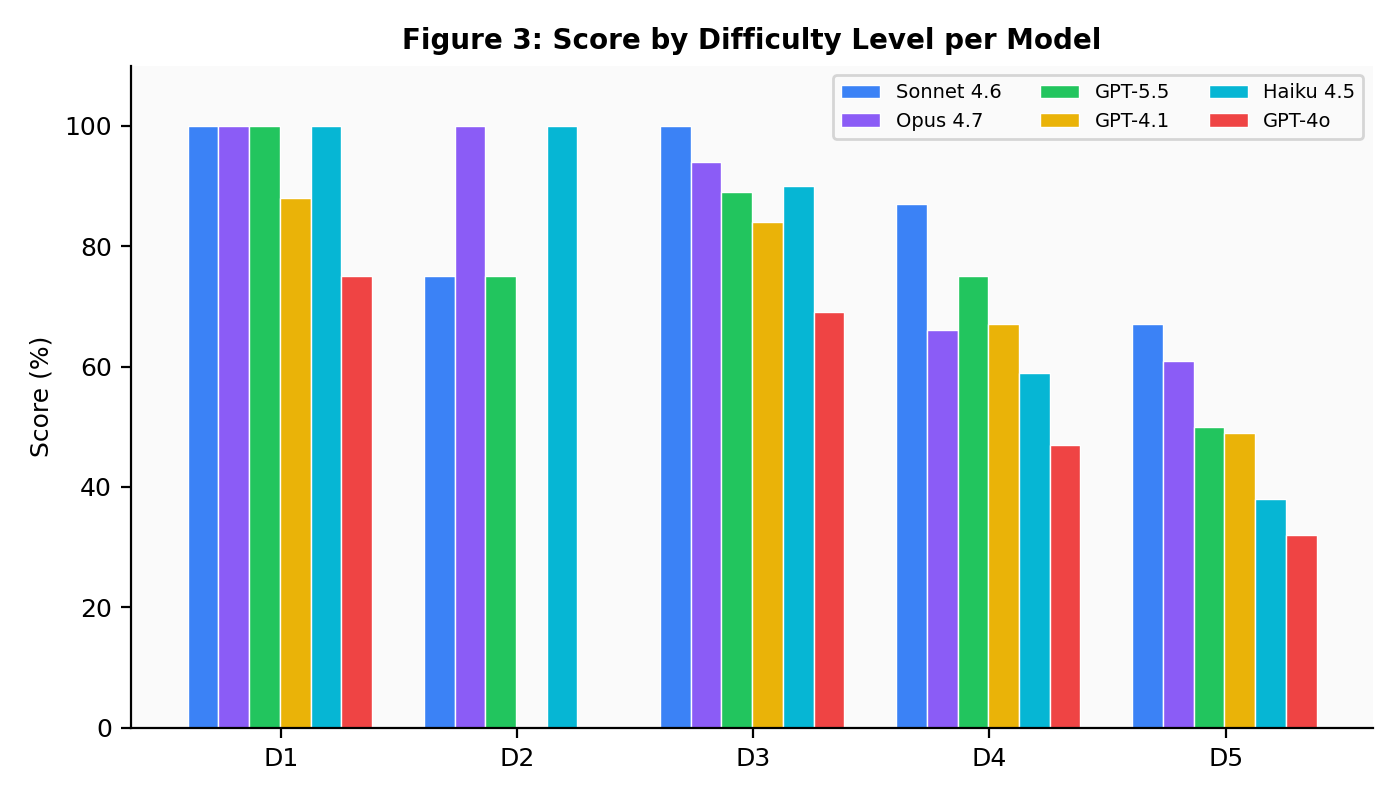
\includegraphics[width=\columnwidth]{fig3_difficulty_per_model.png}}
\caption{Score by difficulty level per model. D4--D5 tasks produce the most differentiation. GPT-4.1 and GPT-4o score 0\% on D2 due to missing a subtle gap.}
\label{fig:difficulty}
\end{figure}

\subsection{Performance by Control Domain}

Fig.~\ref{fig:heatmap} shows the model-control performance matrix. Change Management (CC8.1) is the easiest domain (88\% average), with procedural, well-defined gaps in structured evidence. Vendor Management (CC9.1, 46\%) and Risk Assessment (CC3.1, 43\%) are the hardest, requiring domain-specific knowledge and materiality judgment.

\begin{figure}[htbp]
\centerline{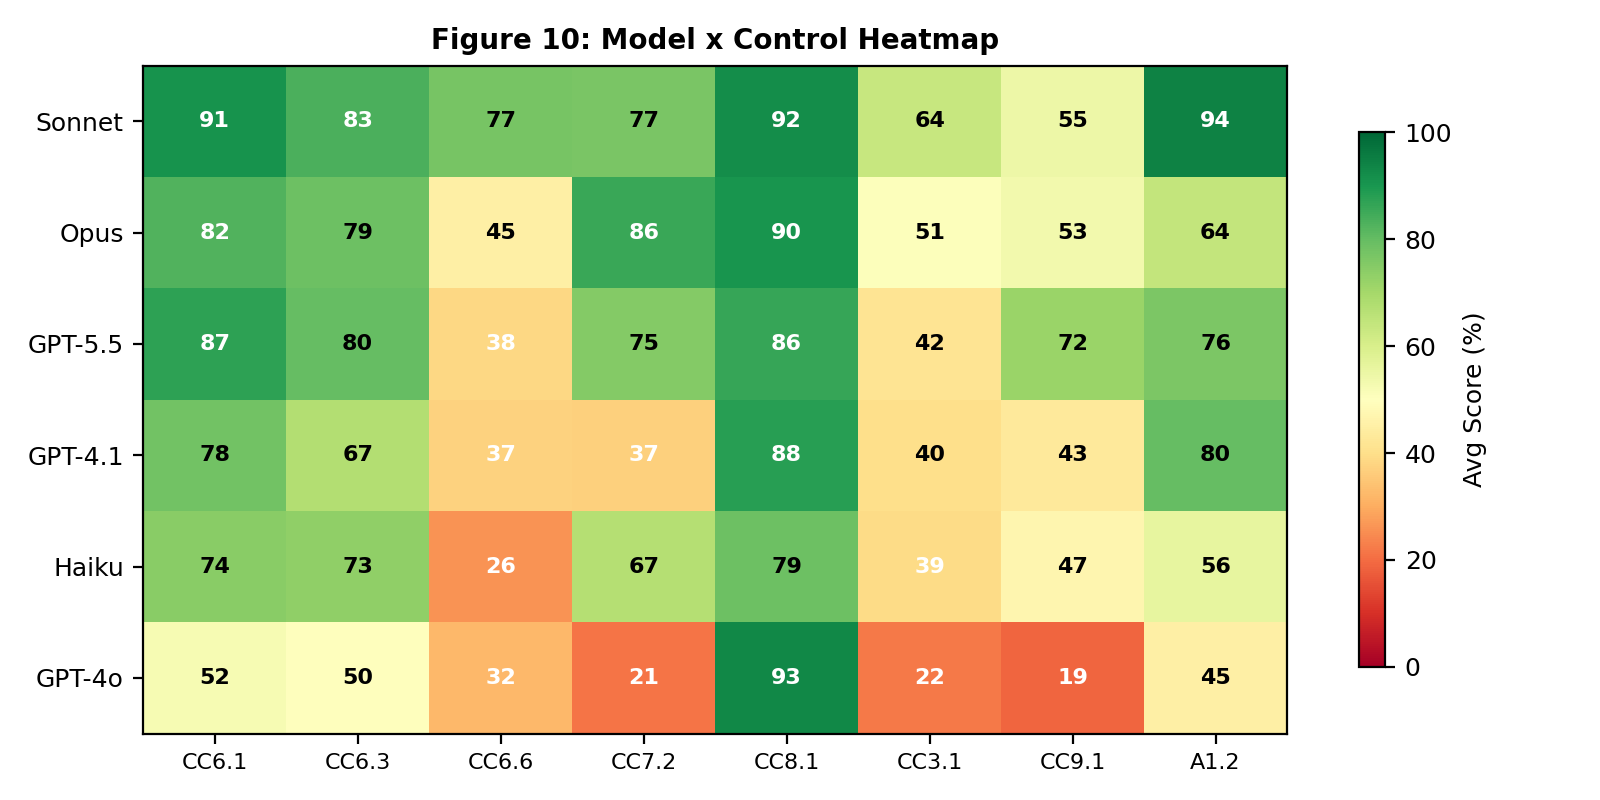
\includegraphics[width=\columnwidth]{fig10_heatmap.png}}
\caption{Model $\times$ Control heatmap. CC8.1 (Change Mgmt) is consistently easiest. CC9.1 and CC3.1 are consistently hardest. CC6.6 shows the widest model variance.}
\label{fig:heatmap}
\end{figure}

\subsection{D5 Judgment Tasks}

Three D5 tasks average below 28\% across all models:

\begin{itemize}
\item \textbf{cc3.1-5-001} (Risk Assessment, 23\%): Risk downgrades without documented justification, 11-month-old annual assessment, partial governance review scope.
\item \textbf{cc9.1-5-001} (Vendor Management, 24\%): Vendor met 72-hour SLA but three-week uncertainty on customer data exposure. Qualified SOC~2 opinion acknowledged without risk assessment.
\item \textbf{cc6.6-5-001} (System Boundaries, 28\%): Admin API bypasses the API gateway---VPN-restricted, accepted risk in penetration test, 0.3\% of traffic.
\end{itemize}

\begin{figure}[htbp]
\centerline{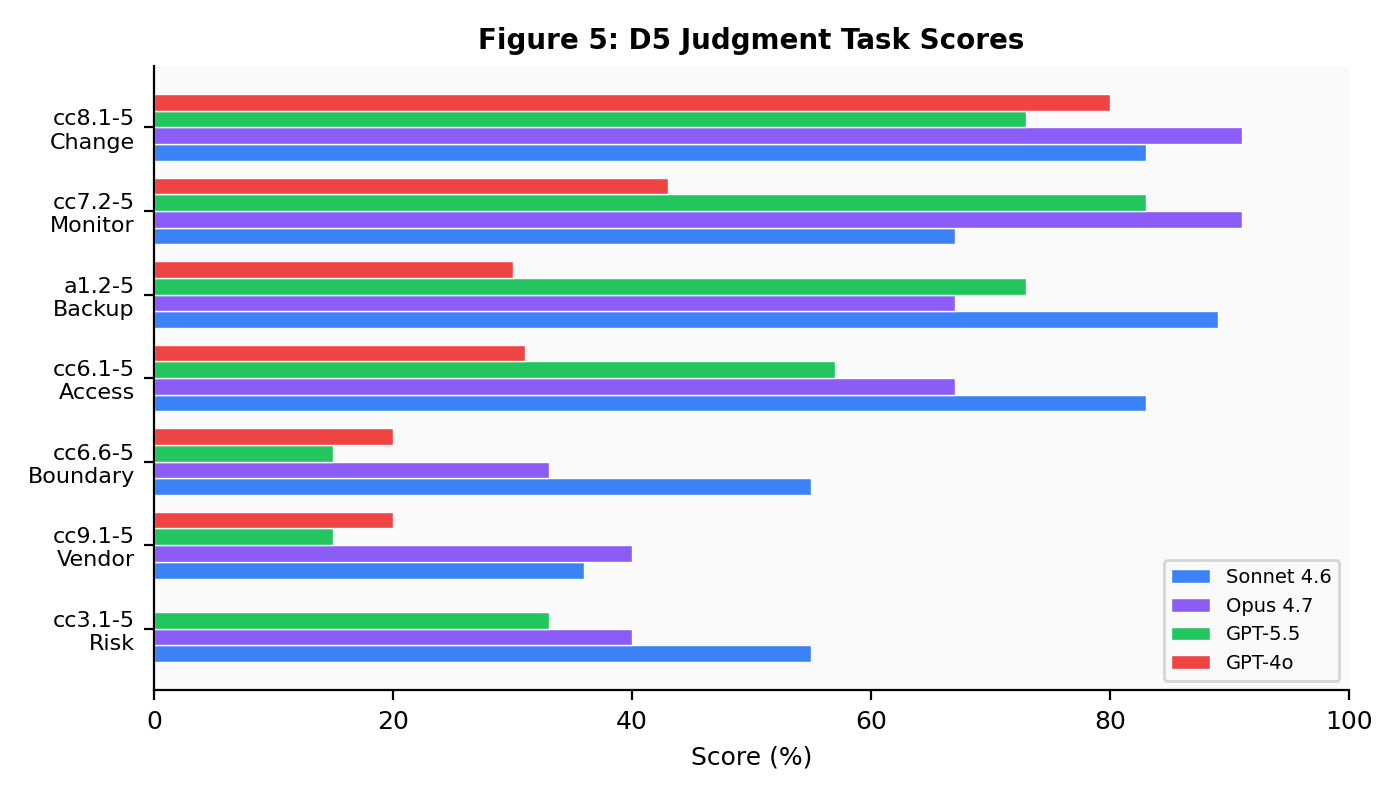
\includegraphics[width=\columnwidth]{fig5_d5_tasks.png}}
\caption{D5 task scores by model. No model exceeds 40\% on the three hardest tasks. Opus leads on Change Management judgment (91\%).}
\label{fig:d5}
\end{figure}

\section{Analysis}

\subsection{Recall Is Commodity; Precision Differentiates}

Most frontier models achieve high recall---they find the planted gaps. The differentiator is precision: how many additional findings the model reports. Haiku~4.5 averages 14.6 findings per task (the highest) but achieves only 39\% precision. Sonnet reports 7.3 findings per task with 63\% precision. Gap detection is approaching commodity status among frontier models; the value lies in calibrated reporting.

\begin{figure}[htbp]
\centerline{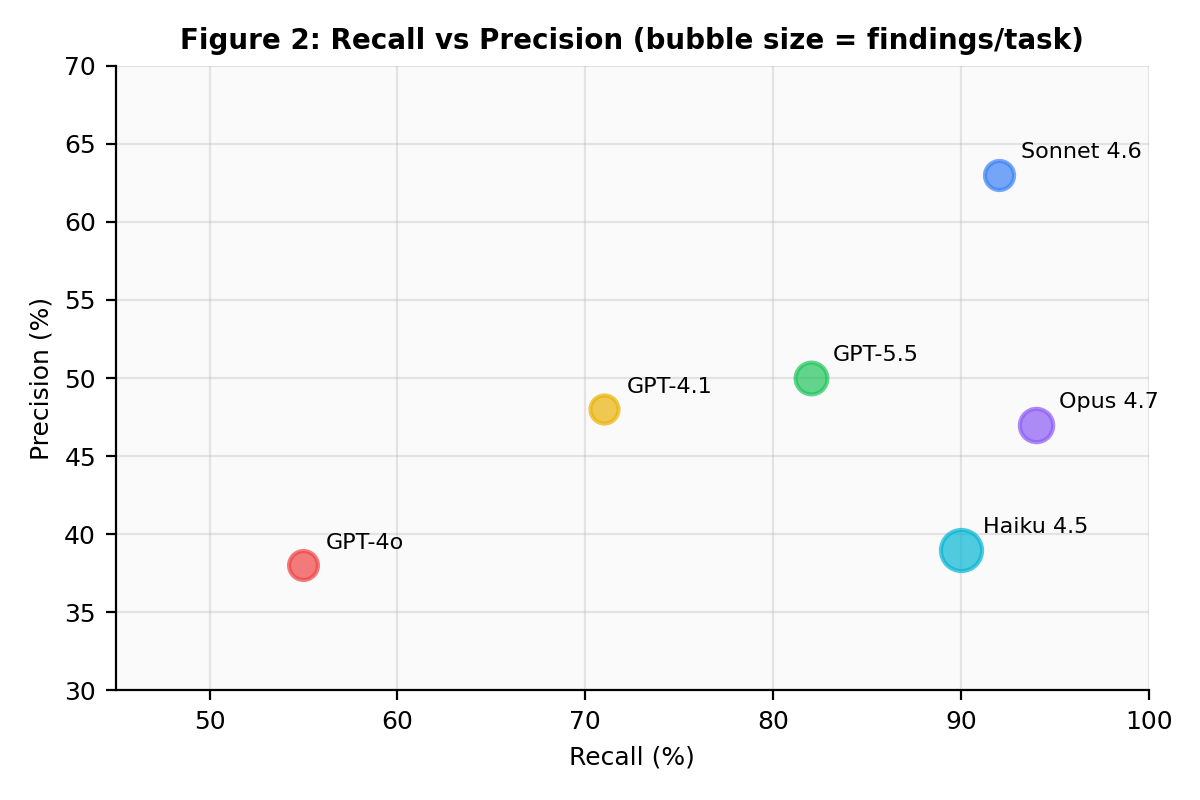
\includegraphics[width=\columnwidth]{fig2_recall_precision.png}}
\caption{Recall vs.\ Precision (bubble size = avg findings/task). Opus achieves the highest recall (94\%) but lowest precision (47\%).}
\label{fig:rp}
\end{figure}

\subsection{The Over-Reporting Penalty}
\label{sec:overreporting}

F1 scoring penalizes models that report findings beyond the planted ground truth. Opus reports 9.6 findings per task on average. The extra findings frequently include observations a human auditor would consider valid: ``emergency approval via Slack DM lacks audit trail,'' ``standard change deployed outside maintenance window.'' Under keyword scoring, these count as false positives.

Sonnet's 10-point lead over Opus (82\% vs.\ 72\%) is partly attributable to this effect. Sonnet also has genuinely higher recall on more D4--D5 tasks (100\% on 16 of 20 tasks vs.\ fewer for Opus), so the lead is not purely an artifact. However, under a scorer that credits legitimate extra findings, the gap between models would narrow.

This limitation is inherent to ground-truth benchmarking for open-ended tasks. Unlike code evaluation (tests pass or fail) or CTF challenges (flag matches or does not), compliance findings exist on a spectrum of validity. A secondary scorer using LLM-as-judge could evaluate extra findings but introduces non-determinism.

\subsection{Domain-Specific Capabilities}

Performance varies by control domain (Fig.~\ref{fig:heatmap}). GPT-4o scores 93\% on Change Management but 19\% on Vendor Management. This suggests compliance capability is not a single dimension but a set of domain-specific competencies. Change Management evidence (structured CSVs, clear policy rules) maps well to LLM pattern matching. Vendor Management requires SOC~2-specific knowledge about subservice organization carve-out methodology and judgment about vendor incident response adequacy.

\section{Limitations}

\begin{itemize}
\item \textbf{Scale.} 20 tasks provides directional findings but lacks statistical power for fine-grained model comparisons.
\item \textbf{Keyword scoring.} Cannot capture all valid phrasings and penalizes legitimate extra findings.
\item \textbf{Synthetic evidence.} Documents are authored, not sourced from real audits.
\item \textbf{Single framework.} All tasks cover SOC~2.
\item \textbf{Single run.} Non-deterministic model outputs introduce variance.
\end{itemize}

\section{Future Work}

\textbf{Task expansion.} Target: 64+ tasks (8 per control). The authoring guide and schema are designed for community contributions.

\textbf{Multi-framework support.} ISO~27001 Annex~A, HIPAA Security Rule, and PCI-DSS v4.0 task sets. The schema supports these without evaluation harness changes.

\textbf{LLM-as-judge.} An optional secondary scorer to evaluate whether extra findings are legitimate compliance observations. The primary keyword score remains for determinism.

\textbf{Scoring research.} The over-reporting penalty is the most significant limitation. Alternatives include expanded ground truth, strict/lenient scoring modes, and human auditor panels.

\section{Related Work}

\textbf{Code benchmarks.} HumanEval~\cite{humaneval} introduced function-level evaluation. SWE-bench~\cite{swebench} extended to real GitHub issues. SWE-bench Pro~\cite{swebenchpro} added contamination resistance across 1,865 tasks.

\textbf{Cybersecurity benchmarks.} CyBench~\cite{cybench} evaluates CTF challenges with subtask decomposition. CyberGym~\cite{cybergym} uses 1,507 real CVEs for PoC generation.

\textbf{Compliance benchmarks.} AIReg-Bench~\cite{aireg} tests EU AI Act compliance (120 samples). LegalBench~\cite{legalbench} tests legal reasoning (162 tasks). CUAD~\cite{cuad} tests contract extraction. None test multi-document compliance auditing.

\textbf{General reasoning.} GAIA~\cite{gaia} tests multi-step reasoning. GPQA~\cite{gpqa} tests graduate-level knowledge. Both use exact-match evaluation.

TrustBench is distinguished by testing compliance-specific skills: multi-document cross-referencing, exception validation, noise filtering, and materiality judgment.

\section{Conclusion}

TrustBench demonstrates that LLMs can detect compliance gaps requiring cross-referencing multiple documents---practical capability for GRC teams. However, no model exceeds 28\% on materiality judgment tasks, models systematically over-report, and performance varies by control domain. We release TrustBench as open-source infrastructure for the compliance AI evaluation ecosystem.

\begin{thebibliography}{00}
\bibitem{swebench} C. E. Jimenez et al., ``SWE-bench: Can Language Models Resolve Real-World GitHub Issues?'' in \textit{Proc. ICLR}, 2024.
\bibitem{swebenchpro} Scale AI, ``SWE-bench Pro: Raising the Bar for Agentic Coding,'' 2025.
\bibitem{cybench} A. K. Zhang et al., ``Cybench: A Framework for Evaluating Cybersecurity Capabilities and Risks of Language Models,'' in \textit{Proc. ICLR}, 2025.
\bibitem{cybergym} Z. Wang et al., ``CyberGym: Evaluating AI Agents on Real-World Vulnerability Analysis,'' \textit{arXiv:2506.02548}, 2025.
\bibitem{aireg} T. Sherborne et al., ``AIReg-Bench: Benchmarking LLMs for AI Regulatory Compliance Assessment,'' 2025.
\bibitem{legalbench} N. Guha et al., ``LegalBench: A Collaboratively Built Benchmark for Measuring Legal Reasoning in Large Language Models,'' in \textit{Proc. NeurIPS}, 2023.
\bibitem{cuad} D. Hendrycks et al., ``CUAD: An Expert-Annotated NLP Dataset for Legal Contract Review,'' in \textit{Proc. NeurIPS}, 2021.
\bibitem{gaia} G. Mialon et al., ``GAIA: A Benchmark for General AI Assistants,'' in \textit{Proc. ICLR}, 2024.
\bibitem{gpqa} D. Rein et al., ``GPQA: A Graduate-Level Google-Proof Q\&A Benchmark,'' \textit{arXiv:2311.12022}, 2023.
\bibitem{humaneval} M. Chen et al., ``Evaluating Large Language Models Trained on Code,'' \textit{arXiv:2107.03374}, 2021.
\end{thebibliography}

\end{document}
